% ---
% Inicia os anexos
% ---
\begin{anexosenv}

% Imprime uma página indicando o início dos anexos
\partanexos

% ---
\chapter{Conversão \textit{Strokes}-\textit{Flashes}: Teste de Sensibilidade de $\epsilon_{spc}$}
\label{anexo_conversao}

A distância base entre \textit{strokes} $\epsilon_{spc}$ usada no algoritmo DBSCAN para a rede BrasilDAT foi determinada considerando que ela seria mínima (para evitar excesso de agrupamento) desde que o tempo entre \textit{strokes} e entre \textit{flashes} apresentasse uma distribuição unimodal centralizada em no máximo $1\:s$.

A \autoref{flash_stats_multi} mostra as estatísticas do agrupamento de \textit{strokes} em \textit{flashes} para diferentes valores de $\epsilon_{spc}$ usando a base de dados da rede BrasilDAT . O histograma de tempo entre \textit{strokes} (a) mostra uma distribuição unimodal centralizada em aproximadamente $0,1\:s$ cuja contagem aumenta com $\epsilon_{spc}$ (já que a quantidade de \textit{strokes} em um flash também aumenta com $\epsilon_{spc}$); o tempo máximo entre \textit{flashes} também ligeiramente aumenta com $\epsilon_{spc}$, ultrapassando o limite de $500\:ms$ estabelecido por \citeonline{Cummins1998} para $\epsilon_{spc}=5\:km$. O histograma de tempo entre \textit{flashes} (a) mostra uma distribuição bimodal centralizada em aproximadamente 0,2 e $1\:s$ que se torna unimodal centralizada em $1\:s$ com o aumento de $\epsilon_{spc}$. O número máximo de \textit{strokes} por \textit{flash} (b) ligeiramente aumenta com $\epsilon_{spc}$, de 17 para $20\:strokes$. A distância entre \textit{strokes} em um \textit{flash} (c), diretamente influenciada por $\epsilon_{spc}$, mostra uma distribuição unimodal centralizada próxima a zero, com uma maior quantidade de pontos até o valor de $\epsilon_{spc}$ escolhido e alguns pontos com até o dobro da distância $\epsilon_{spc}$; nota-se que, mesmo para $\epsilon_{spc}=5\:km$ (\autoref{flash_stats_5km}), os pontos na distância máxima ainda estão dentro da consideração (b) da \autoref{strokestoflashes} (\textit{strokes} subsequentes em um raio máximo de $50\:km$). Dentro das determinações estipuladas, definiu-se que $\epsilon_{spc}=2,5\:km$ é a escolha mais adequada.

\begin{figure}[hb]
	\begin{center}
		\caption{Histogramas de tempo entre strokes e entre \textit{flashes} (a), número de \textit{strokes} por \textit{flash} (b) e distância latitude e longitudinal entre \textit{strokes} em um \textit{flash} (c) para diferentes valores de $\epsilon_{\text{spc}}$.} 
		\label{flash_stats_multi}
		%		\setcaptionmargin{1cm}
		\subfloat[$\epsilon_{\text{spc}}=1\:km$]{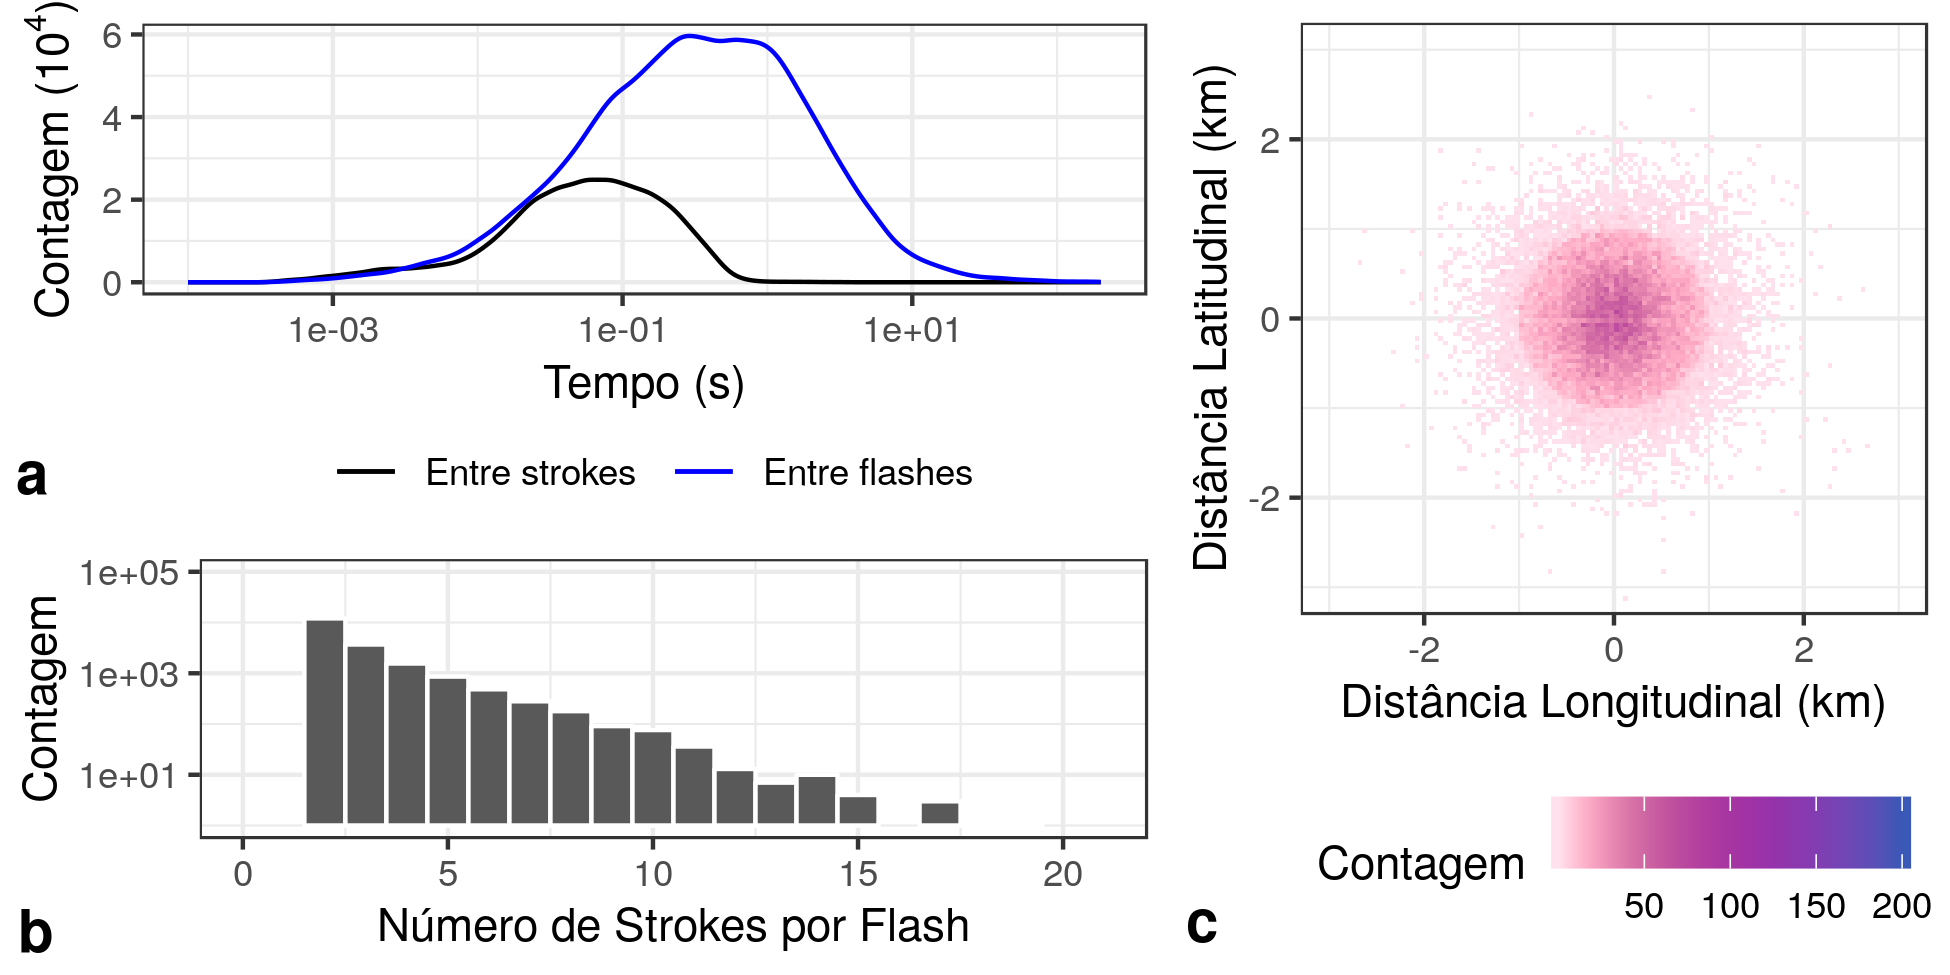
\includegraphics[width=\columnwidth]{../Lightning_Processing/figures/brasildat_flash_stats_1km_ptbr.png}
			\label{flash_stats_1km}} \\
		\subfloat[$\epsilon_{\text{spc}}=2,5\:km$]{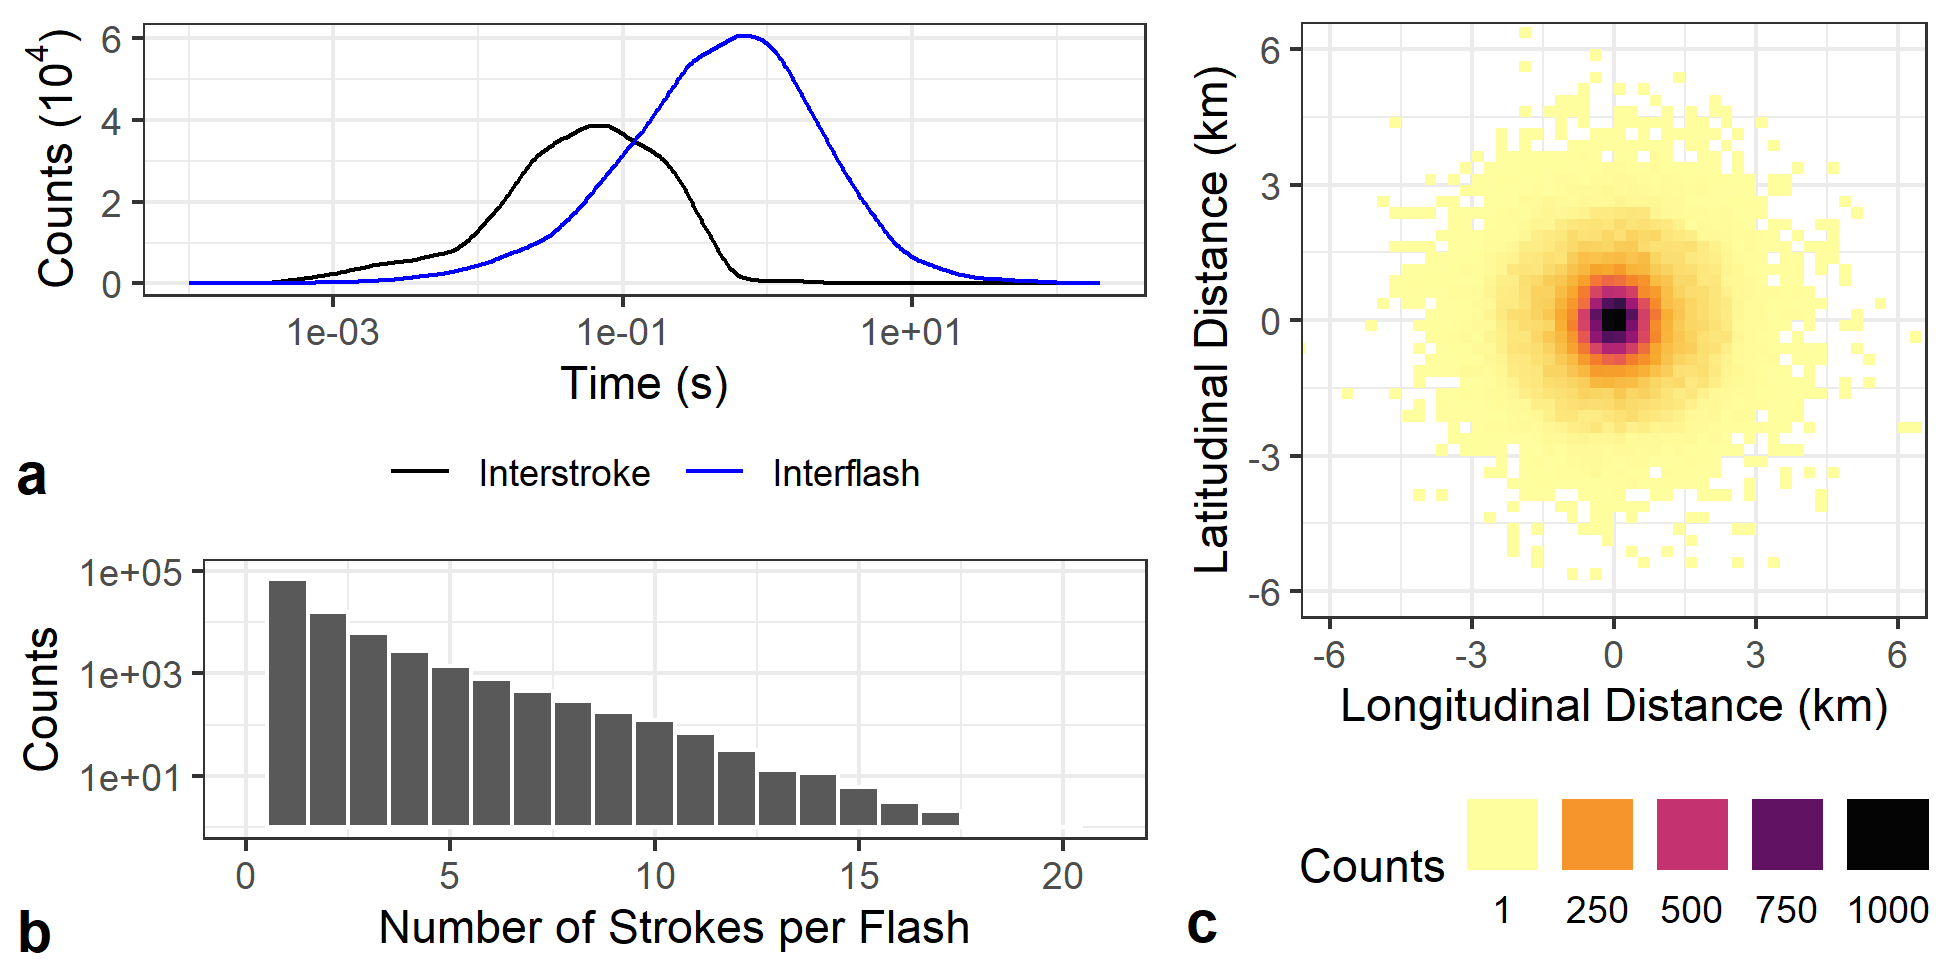
\includegraphics[width=\columnwidth]{../Lightning_Processing/figures/brasildat_flash_stats_ptbr.png}
			\label{flash_stats_2.5km}} \\
		\legend{Fonte: Produzido pela autora.}
	\end{center}
\end{figure}
\clearpage
\begin{figure}[ht]\ContinuedFloat
	\begin{center}
		\caption{\textit{Continuação}.}
		\subfloat[$\epsilon_{\text{spc}}=5\:km$]{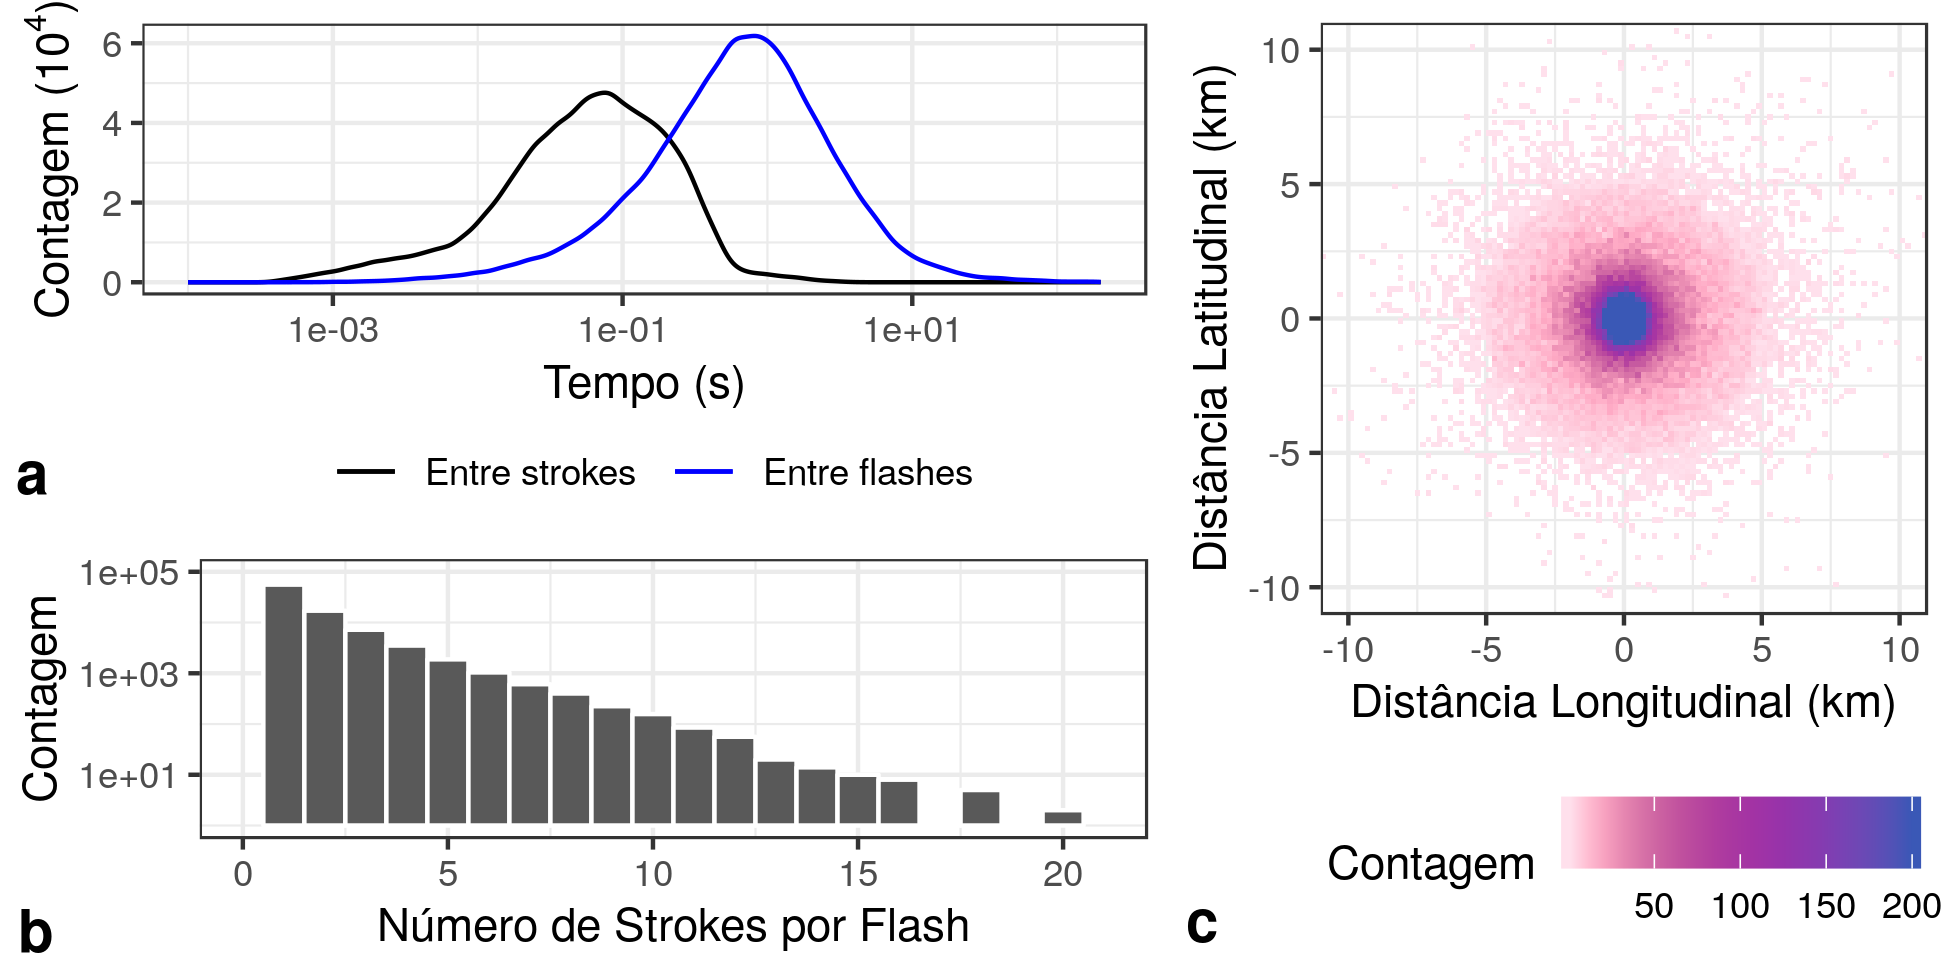
\includegraphics[width=\columnwidth]{../Lightning_Processing/figures/brasildat_flash_stats_5km_ptbr.png}
			\label{flash_stats_5km}} \\
		\legend{Fonte: Produzido pela autora.}
	\end{center}
\end{figure}

\end{anexosenv}
